


\subsection{Grid Options}
	
\begin{pgfplotsxykeylist}{\x minorgrids=\mchoice{true,false} (initially false),\x majorgrids=\mchoice{true,false} (initially false),grid=\mchoice{minor,major,both,none} (initially false)}
Enables/disables different grid lines. Major grid lines are placed at the normal tick positions (see |xmajorticks|) while minor grid lines are placed at minor ticks (see |xminorticks|). 

This example employs the coordinates defined on page~\pageref{page:plotcoords:src}.
\begin{codeexample}[]
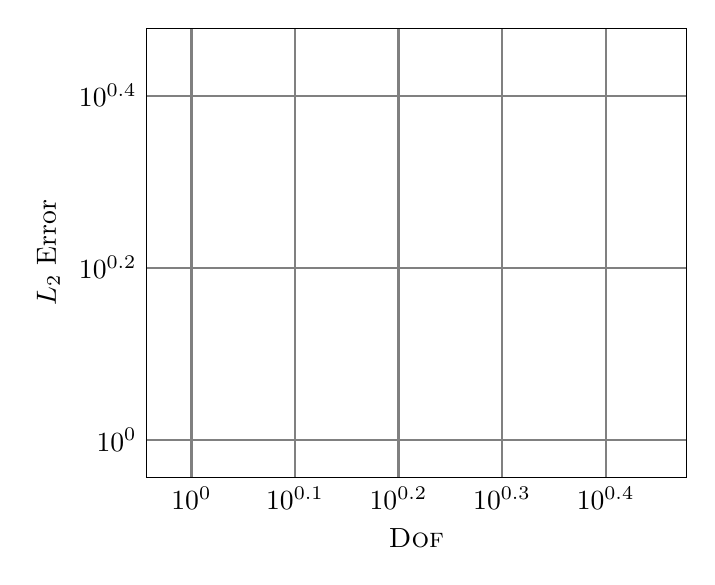
\begin{tikzpicture}
\begin{loglogaxis}[
	xlabel={\textsc{Dof}},
	ylabel={$L_2$ Error},
	grid=major
]
% see above for this macro:
\plotcoords
\end{loglogaxis}
\end{tikzpicture}
\end{codeexample}

\begin{codeexample}[]
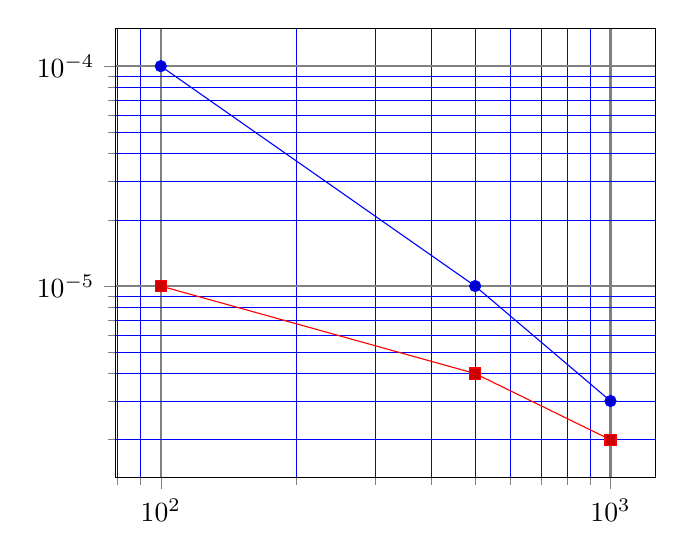
\begin{tikzpicture}
\begin{loglogaxis}[
	grid=both,
	tick align=outside,
	tickpos=left]
\addplot coordinates 
	{(100,1e-4) (500,1e-5) (1000,3e-6)};
\addplot coordinates 
	{(100,1e-5) (500,4e-6) (1000,2e-6)};
\end{loglogaxis}
\end{tikzpicture}
\end{codeexample}

Grid lines will be drawn before tick lines are processed, so ticks will be drawn on top of grid lines. You can configure the appearance of grid lines with the styles
\begin{codeexample}[code only]
\pgfplotsset{grid style={help lines}} % modifies the style `every axis grid'
\pgfplotsset{minor grid style={color=blue}} % modifies the style `every minor grid'
\pgfplotsset{major grid style={thick}} %modifies the style `every major grid'
\end{codeexample}
\end{pgfplotsxykeylist}


\subsection{Custom Annotations}
Often, one may want to add custom drawing elements or descriptive texts to an axis. These graphical elements should be associated to some logical coordinate, grid point, or perhaps they should just be placed somewhere into the axis.

\PGFPlots\ assists with the following ways when it comes to annotations:
\begin{enumerate}
	\item You can explicitly provide any \Tikz\ instruction like |\draw ... ;| into the axis. Here, the |axis cs| allows
	to provide coordinates of \PGFPlots.

	Furthermore, |rel axis cs| allows to position \Tikz\ elements relatively (like ``$50\%$ of the axis' width).
	\item \PGFPlots\ can automatically generate nodes at every coordinate using its |nodes near coords| feature.
	%\item \PGFPlots\ can automatically generate \Tikz\ labels for every coordinate (FIXME).
	\item \PGFPlots\ allows you to place nodes on a plot, using the |\addplot ... node[pos=|\meta{fraction}|] {};| feature.
\end{enumerate}
This section explains all of the approaches, except for the |nodes near coords| feature which is documented in its own section.

\subsubsection{Accessing Axis Coordinates in Graphical Elements}
\label{sec:axis:coords}%
\begin{coordinatesystem}{axis cs}
\PGFPlots\ provides a new coordinate system for use inside of an axis, the ``axis coordinate system'', |axis cs|.

It can be used to draw any \Tikz-graphics at axis coordinates. It is used like
\begin{codeexample}[code only]
\draw 
   (axis cs:18943,2.873391e-05) 
|- (axis cs:47103,8.437499e-06);
\end{codeexample}
\begin{codeexample}[]
\tikzstyle{every pin}=[fill=white,
	draw=black,
	font=\footnotesize]
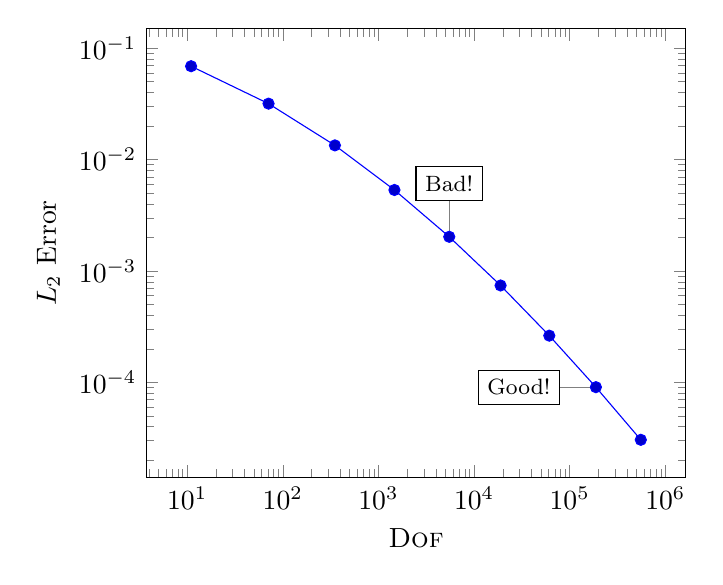
\begin{tikzpicture}
	\begin{loglogaxis}[
		xlabel={\textsc{Dof}},
		ylabel={$L_2$ Error}]

	\addplot coordinates {
		(11,     6.887e-02)
		(71,     3.177e-02)
		(351,    1.341e-02)
		(1471,   5.334e-03)
		(5503,   2.027e-03)
		(18943,  7.415e-04)
		(61183,  2.628e-04)
		(187903, 9.063e-05)
		(553983, 3.053e-05)
	};

	\node[coordinate,pin=above:{Bad!}] 
		at (axis cs:5503,2.027e-03) {};
	\node[coordinate,pin=left:{Good!}] 
		at (axis cs:187903,9.063e-05)	{};
	\end{loglogaxis}
\end{tikzpicture}
\end{codeexample}

\begin{codeexample}[]
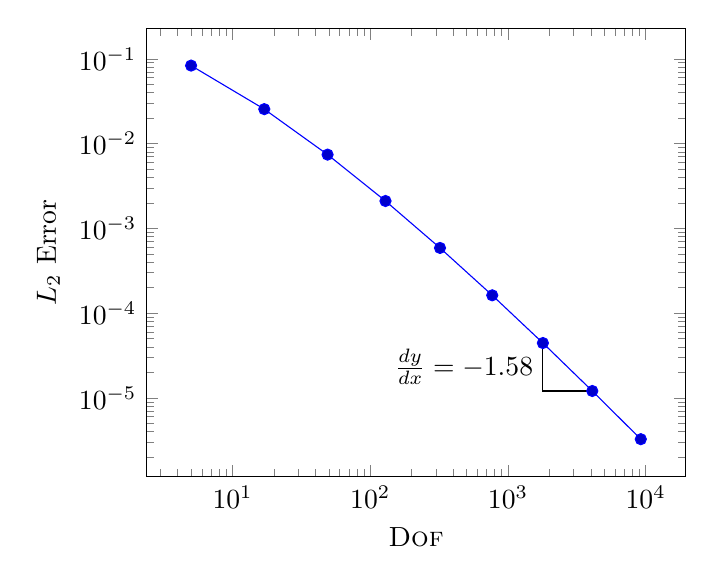
\begin{tikzpicture}
\begin{loglogaxis}[
	xlabel=\textsc{Dof},
	ylabel=$L_2$ Error
]
\draw 
		(axis cs:1793,4.442e-05)
	|-  (axis cs:4097,1.207e-05)
	node[near start,left] 
	{$\frac{dy}{dx} = -1.58$};

\addplot coordinates {
	(5,    8.312e-02)
	(17,   2.547e-02)
	(49,   7.407e-03)
	(129,  2.102e-03)
	(321,  5.874e-04)
	(769,  1.623e-04)
	(1793, 4.442e-05)
	(4097, 1.207e-05)
	(9217, 3.261e-06)
};
\end{loglogaxis}
\end{tikzpicture}
\end{codeexample}

Whenever you draw additional graphics, consider using |axis cs|! It applies any custom transformations (including |symbolic x coords|), logarithms, data scaling transformations or whatever \PGFPlots\ usually does and provides a low level \pgfname\ coordinate as result.

In case you need only one component (say, the $y$ component) of such a vector, you can use the |\pgfplotstransformcoordinatey| command, see Section~\ref{sec:basic:coordinates} for details about basic level access.

The result of |axis cs| is always an absoute position inside of an axis. This means, in particular, that \emph{adding} two points has unexpected effects: the expression |(axis cs:0,0) ++ (axis cs:1,0)| is not necessarily the same as |(axis cs:1,0)|. The background for such unexpected effects is that \PGFPlots\ applies a \emph{shifted} linear transformation which moves the origin in order to support its high accuracy and high data range (compare the documentation of |disabledatascaling|).

In order to express \emph{relative} positions (or lengths), you need to use |axis direction cs|.
\end{coordinatesystem}

\begin{coordinatesystem}{axis direction cs}
	While |axis cs| allows to supply \emph{absolute positions}, |axis direction cs| supplies \emph{directions}. It allows to express \emph{relative} positions, includings lengths and dimensions, by means of axis coordinates.

	As noted in the documentation for |axis cs|, adding two coordinates by means of the \tikzname\ |++| operator may have unexpected effects. The correct way for |++| operations is |axis direction cs|:
\begin{codeexample}[]
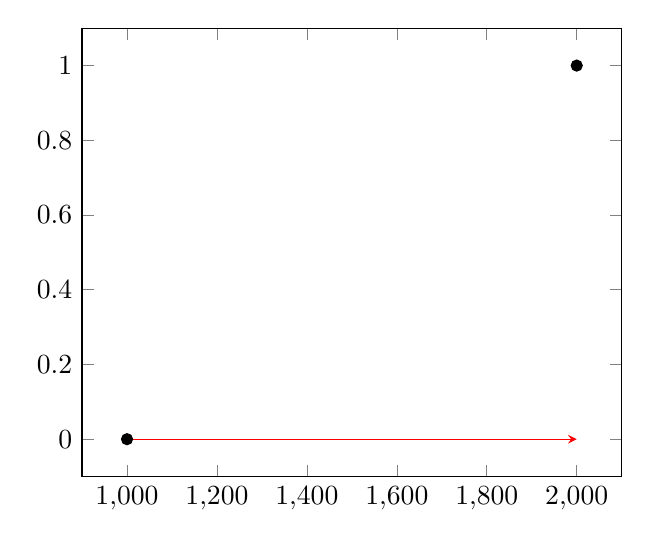
\begin{tikzpicture}
\begin{axis}
	\draw[red,-stealth] 
		(axis cs:1000,0) 
		-- % = line-to
	 	++ % = calculate a vector sum
	    (axis direction cs:1000,0);

	\addplot [only marks,mark=*] 
		coordinates { (1000,0) (2000,1) };
\end{axis}
\end{tikzpicture}
\end{codeexample}
	\noindent Here, the target of the red arrow is the position |(axis cs:2000,0)| as expected.

	Using relative positions is mainly useful for linear axes. Applying this command to log-axes might still work, but it requires more care.

	One use-case is to supply lengths -- for example in order to support |circle| or |ellipse| paths. The correct way to draw an ellipse in \PGFPlots\ would be to specify the two involved radii by means of two |(axis direction cs:|\meta{x,y}|)| expressions. In general, this is possible if you use the basic level macros |\pgfpathellipse| and |\pgfplotspointaxisdirectionxy|. Please refer to the documentation of |\pgfplotspointaxisdirectionxy| for two examples of drawing arbitrary ellipses by means of this method. 
	
	Since drawing circles and ellipses inside of an axis is a common use-case, \PGFPlots\ automatically communicates its coordinate system transformations to \tikzname: whenever you write |\draw ellipse[|\declareandlabel{x radius}|=|\meta{x}|,|\declareandlabel{y radius}|=|\meta{y}|]|, the arguments \meta{x} and \meta{y} are considered to be \PGFPlots\ direction vectors and are handed over to |axis direction cs|. Consequently, ellipses with axis parallel radii are straight-forward and use the normal \tikzname\ syntax:
\begin{codeexample}[]
% requires \pgfplotsset{compat=1.5.1} !
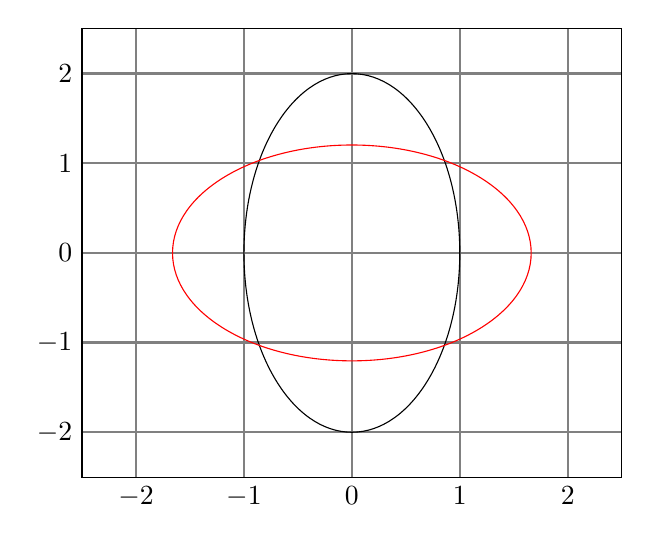
\begin{tikzpicture}
\begin{axis}[
	xmin=-2.5,   xmax=2.5,
	ymin=-2.5,   ymax=2.5,
	xtick={-2,-1,0,1,2},
	ytick={-2,-1,0,1,2},
	grid=major,
]
	% standard tikz syntax:
	\draw[black] (axis cs:0,0)
		ellipse [
			x radius=1, y radius=2];

	\draw[red]   (axis cs:0,0)
		ellipse [rotate=90,
			x radius=1, y radius=2];
	% see \pgfplotspointaxisdirectionxy 
	% for arbitrary ellipses
\end{axis}
\end{tikzpicture}
\end{codeexample}
	Here, the two ellipses are specified as usual in \tikzname. \PGFPlots\ ensures that all necessary transformations are applied to the two radii. Note that \PGFPlots\ usually has different axis scales for $x$~and~$y$. As a consequence, the rotated red ellipse does not fit into the axis lines; we would need to use |axis equal| to allow properly rotated ellipses.

	\paragraph{Attention:} this modification to circles and ellipses requires |\pgfplotsset{compat=1.5.1}|.

	The same applies to circles: in the standard view, a circle with \declareandlabel{radius}|=|$r$ will appear as an ellipse due to the different axis scales. Supplying |axis equal| results in true circles:
\begin{codeexample}[]
% requires \pgfplotsset{compat=1.5.1} !
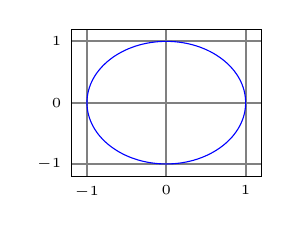
\begin{tikzpicture}
\begin{axis}[tiny,enlargelimits,
	xmin=-1,xmax=1,
	ymin=-1,ymax=1,
	xtick={-1,0,1},
	ytick={-1,0,1},
	grid=major,
]
	\draw[blue] (axis cs:0,0) circle[radius=1];
\end{axis}
\end{tikzpicture}
\end{codeexample}
\begin{codeexample}[]
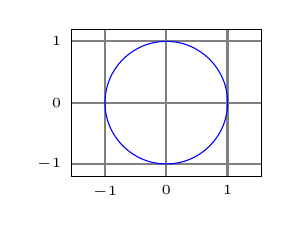
\begin{tikzpicture}
\begin{axis}[tiny,enlargelimits,
	axis equal,
	xmin=-1,xmax=1,
	ymin=-1,ymax=1,
	xtick={-1,0,1},
	ytick={-1,0,1},
	grid=major,
]
	\draw[blue] (axis cs:0,0) circle[radius=1];
\end{axis}
\end{tikzpicture}
\end{codeexample}

	In case you need access to |axis direction cs| inside of math expressions, you can employ the additional math function \declareandlabel{transformdirectionx}. It does the same as |axis direction cs|, but only in $x$ direction. The result of |transformdirectionx| is a dimensionless unit which can be interpreted relative to the current \pgfname\ $x$ unit vector $e_x$ (see the documentation of |\pgfplotstransformdirectionx| for details).
	There are the math commands |transformdirectionx|, \declareandlabel{transformdirectiony}, and (if the axis is three--dimensional) \declareandlabel{transformdirectionz}. Each of them defines |\pgfmathresult| to contain the result of |\pgfplotstransformdirectionx| (or its variants for $y$ and $z$, respectively).
	
\end{coordinatesystem}


\begin{coordinatesystem}{rel axis cs}
The ``relative axis coordinate system'', |rel axis cs|, uses the complete axis vectors as units. That means `$x=0$' denotes the point on the lower $x$ axis range and `$x=1$' the point on the upper $x$ axis range (see the remark below for |x dir=reverse|).

\pgfplotsexpensiveexample
\begin{codeexample}[]
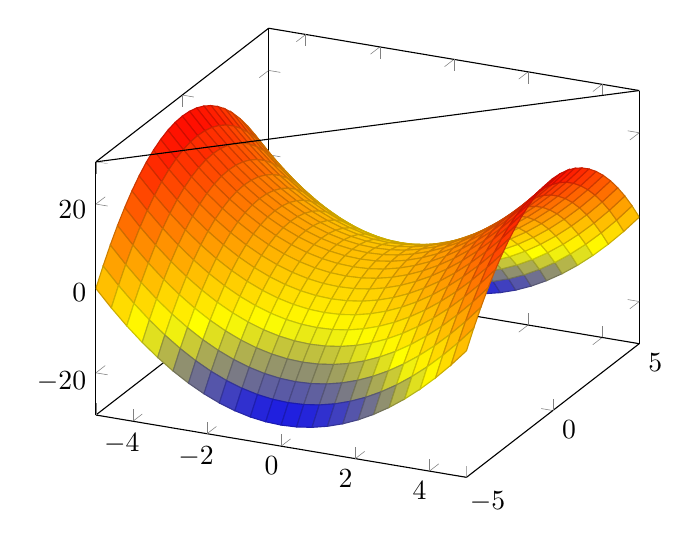
\begin{tikzpicture}
\begin{axis}

	\addplot3[surf] {x^2 - y^2};
	\draw  (rel axis cs:0,0,1) 
		-- (rel axis cs:1,1,1);
\end{axis}
\end{tikzpicture}
\end{codeexample}

\pgfplotsexpensiveexample
\begin{codeexample}[]
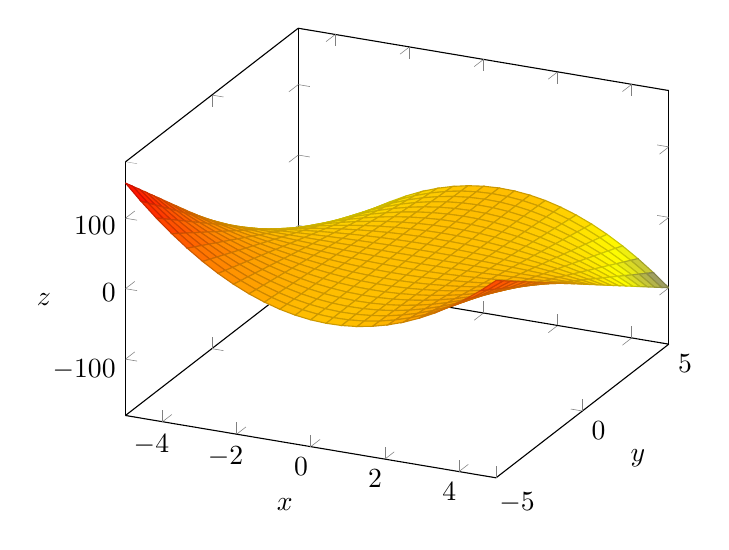
\begin{tikzpicture}
\begin{axis}[
	xlabel=$x$,
	ylabel=$y$,
	zlabel=$z$,
	every axis x label/.style={
		at={(rel axis cs:0.5,-0.15,-0.15)}},
	every axis y label/.style={
		at={(rel axis cs:1.15,0.5,-0.15)}},
	every axis z label/.style={
		at={(rel axis cs:-0.15,-0.15,0.5)}},
]

	\addplot3[surf] {x*(1-x)*y};
\end{axis}
\end{tikzpicture}
\end{codeexample}

	Points identified by |rel axis cs| use the syntax

		|(rel axis cs:|\meta{x}|,|\meta{y}|)| or

		|(rel axis cs:|\meta{x}|,|\meta{y}|,|\meta{z}|)| 
	
	\noindent where \meta{x}, \meta{y} and \meta{z} are coordinates or constant mathematical expressions. The second syntax is only available in three dimensional axes.

	There is one specialty: if you reverse an axis (with |x dir=reverse|), points provided by |rel axis cs| will be \emph{unaffected} by the axis reversal. This is intended to provide consistent placement even for reversed axes. Use |allow reversal of rel axis cs=false| to disable this feature.

There is also a low--level interface to access the transformations and coordinates, see Section~\ref{sec:pgfplots:lowlevel} on page~\pageref{sec:pgfplots:lowlevel}.
\end{coordinatesystem}

\begin{predefinednode}{current plot begin}
	This coordinate will be defined for every plot and can be used is \meta{trailing path commands} or after a plot. It is the first coordinate of the current plot.	
\end{predefinednode}

\begin{predefinednode}{current plot end}
	This coordinate will be defined for every plot. It is the last coordinate of the current plot.	
\end{predefinednode}

\begin{pgfplotskey}{allow reversal of rel axis cs=\mchoice{true,false} (initially true)}
	A fine-tuning key which specifies how to deal with |x dir=reverse| and |rel axis cs| and |ticklabel cs|.

	The initial configuration |true| means that points placed with |rel axis cs| and/or |ticklabel cs| will be at the same position inside of the axes even if its ordering has been reversed. The choice |false| will disable the special treatment of |x dir=reverse|.
\end{pgfplotskey}

\subsubsection{Placing Nodes on Coordinates of a Plot}
{
\tikzset{external/figure name/.add={}{nodes_}}%
The |\addplot| command is not only used for \PGFPlots, it can also carry additional drawing instructions which are handed over to \Tikz\ after the plot's path is complete. Among others, this can be used to add further nodes on the path.

\begin{key}{/tikz/pos=\marg{fraction}}
	The \meta{fraction} identifies a part of the recently completed plot if it is used before the trailing semicolon:
\pgfplotsexpensiveexample
\begin{codeexample}[]
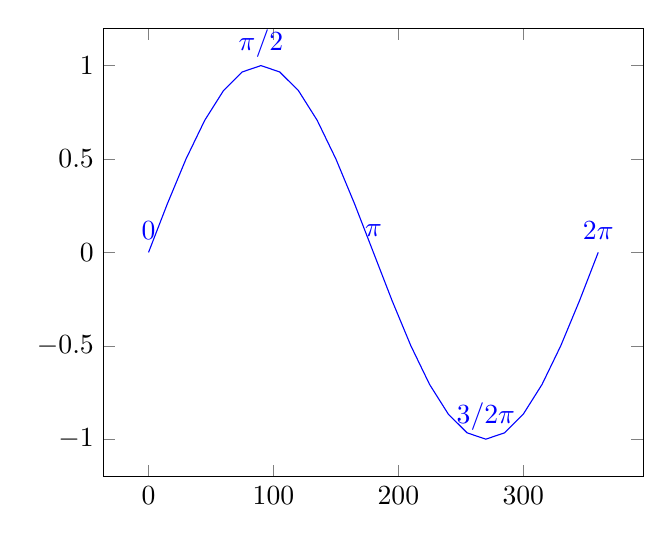
\begin{tikzpicture}
	\begin{axis}
	\addplot[blue,domain=0:360] {sin(x)} 
	[yshift=8pt]
		node[pos=0] {$0$} 
		node[pos=0.25] {$\pi/2$}
		node[pos=0.5] {$\pi$}
		node[pos=0.75] {$3/2\pi$}
		node[pos=1] {$2\pi$}
	;
	\end{axis}
\end{tikzpicture}
\end{codeexample}
\noindent Here, the |[yshift=8pt]| tells \Tikz\ to shift all following nodes upwards. The |node[pos=0] {$0$}| instruction tells \Tikz\ to add a text node at $0\%$ of the recently completed plot. The relative position $0\%$ (|pos=0|) refers to the first coordinate which has been seen by \PGFPlots, and $100\%$ (|pos=1|) refers to the last coordinate. Any value between $0$ and $1$ is interpolated in-between. Note that all these nodes belong to the plot's visualization (which is terminated by the semicolon). Consequently, all these nodes inherit the same graphic settings (like color choices).

	The position on the plot is computed by \PGFPlots\ using \emph{logical} coordinates. That means: it computes the overall length of the curve before the curve is projected to screen coordinates and identifies the desired position\footnote{This can be a time-consuming process. Consider using the external library if you have lots of such figures.}. Afterwards, it projects the final position to screen coordinates. Thus, the position identifies a location on the plot which is always the same, even in case of a rotated three-dimensional axis. \PGFPlots\ will linearly interpolate the fraction between successive coordinates.

	Valid choices for \meta{fraction} are any numbers in the range $[0,1]$.

	Note that the precise meaning of |pos| depends on the current plot handler: for most plot handlers, it defaults to linear interpolation (as in the examples above). For |only marks|, |scatter|, |ybar|, |xbar|, |ybar interval|, and |xbar interval|, it snaps to the nearest encountered coordinate. In this context, ``snap to nearest'' means that |pos=|$p$ refers to the coordinate with index $i = \text{round}(p \cdot N)$ where $N$ is the total number of points:
\begin{codeexample}[]
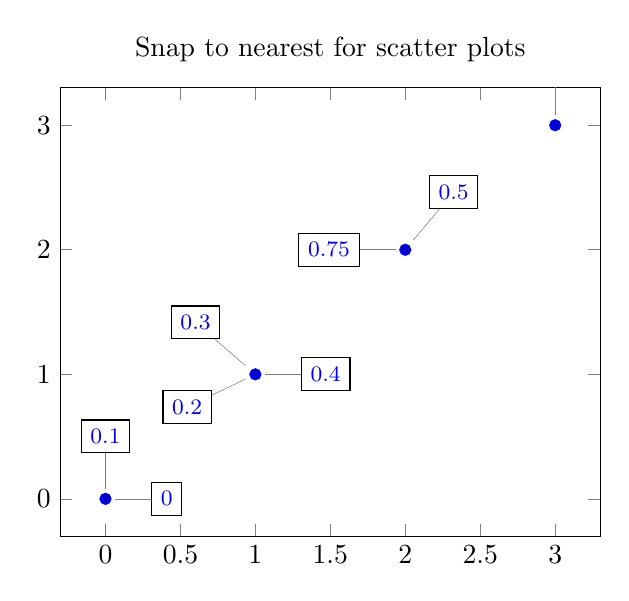
\begin{tikzpicture}
\begin{axis}[title=Snap to nearest for scatter plots]
\addplot+[only marks] 
	coordinates {(0,0) (1,1) (2,2) (3,3)} 
	node[pos=0,   pin=0  :0   ] {}
	node[pos=0.1, pin=90 :0.1 ] {}
	node[pos=0.2, pin=200:0.2 ] {}
	node[pos=0.3, pin=135:0.3 ] {}
	node[pos=0.4, pin=0  :0.4 ] {}
	node[pos=0.5, pin=60 :0.5 ] {}
	node[pos=0.75,pin=180:0.75] {}
	node[pos=1,   pin=90 :1   ] {}
;
\end{axis}
\end{tikzpicture}
\end{codeexample}
	\noindent the previous example shows that |pos=|$p$ maps to one of the four available coordinates, namely the one whose index is closest to $p\cdot N$. Note that in such a case, the distance between coordinates is irrelevant -- only the coordinate index counts.


	Note that the fact that \PGFPlots\ uses \emph{logical} coordinates to compute the target positions can produce unexpected effects if $x$ and $y$ axis operate on a different scales. Suppose, for example, that $x$ is always of order $10^3$ whereas $y$ is of order $10^{-3}$. In such a scenario, the $y$ coordinate have no significant contribution to the curve's length -- although the rescaled axes clearly show ``significant'' $y$ dynamics. Consider using |axis equal| together with |pos| to produce comparable effects.
\end{key}

\begin{key}{/tikz/sloped (initially false)}
	Providing the \Tikz\ key |sloped| to a node identified by |pos| causes it to be rotated such that it adapts to the plot's gradient.
\pgfplotsexpensiveexample
\begin{codeexample}[]
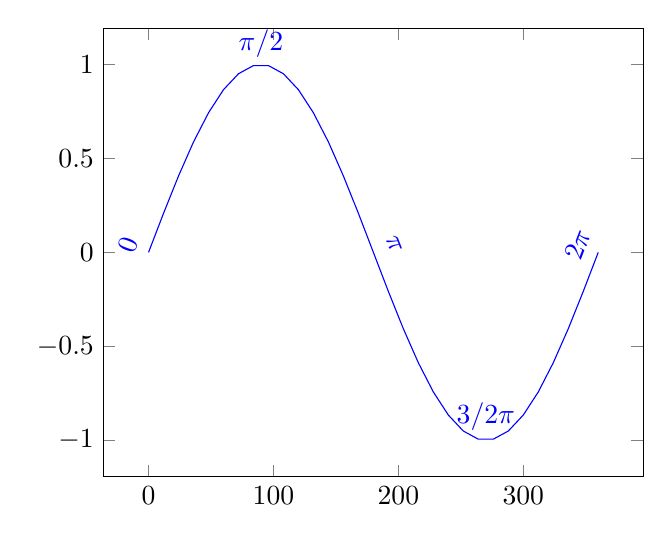
\begin{tikzpicture}
	\begin{axis}
	\addplot[blue,domain=0:360,samples=31] {sin(x)} 
	[every node/.style={yshift=8pt},sloped]
		node[pos=0] {$0$} 
		node[pos=0.25] {$\pi/2$}
		node[pos=0.5] {$\pi$}
		node[pos=0.75] {$3/2\pi$}
		node[pos=1] {$2\pi$}
	;
	\end{axis}
\end{tikzpicture}
\end{codeexample}
	Note that the sequence in which |sloped| and shift transformations are applied is important: if shifts are applied first (as would be the case without the |every node/.style| construction), the shifts do not respect the rotation. If |sloped| is applied first, any subsequent shifts will be applied in the \emph{rotated} coordinates. Thus, the case |every node/.style={yshift=8pt}| shifts every node by |8pt| in direction of its normal vector.

	The |sloped| transformation is based on the gradient between two points (the two points adjacent to |pos|). Consequently, it inherits any sampling weaknesses. To see this, consider the example above with a different number of samples:
\pgfplotsexpensiveexample
\begin{codeexample}[]
% same as above with different number of samples
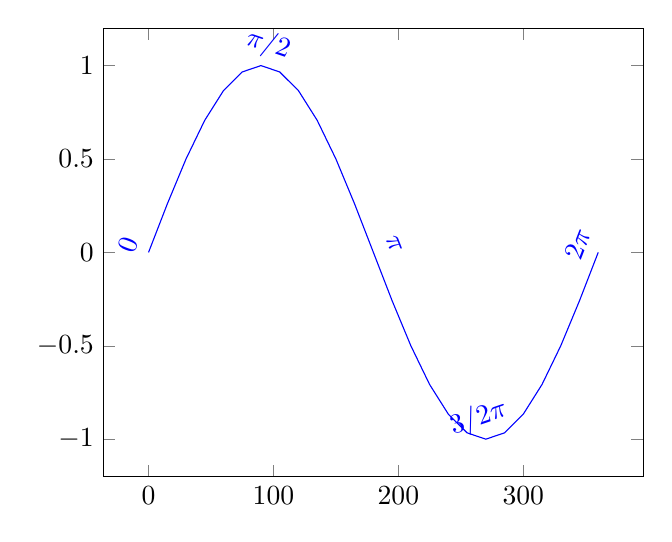
\begin{tikzpicture}
	\begin{axis}
	\addplot[blue,domain=0:360,samples=25] {sin(x)} 
	[every node/.style={yshift=8pt},sloped]
		node[pos=0] {$0$} 
		node[pos=0.25] {$\pi/2$}
		node[pos=0.5] {$\pi$}
		node[pos=0.75] {$3/2\pi$}
		node[pos=1] {$2\pi$}
	;
	\end{axis}
\end{tikzpicture}
\end{codeexample}
	\noindent Here, the two extreme points have small slopes due to the sampling. While this does not seriously affect the quality of the plot, it has a huge impact on the transformation matrizes. Keep this in mind when you work with |sloped| (perhaps it even helps to add a further |rotate| argument).
\end{key}

\begin{key}{/tikz/allow upside down=\mchoice{true,false} (initially false)}
	If |/tikz/sloped| is enabled and one has some difficult line plot, the transformation may cause nodes to be drawn upside down. The default configuration |allow upside down=false| will switch the rotation matrix, whereas |allow upside down| allows this case.
\end{key}

\begin{key}{/tikz/pos segment=\marg{segment index} (initially empty)}
	Occasionally, one has a single plot which consists of multiple segments (like those generated by |empty line=jump| or |contour prepared|). The individual segments will typically have different lengths, so it is tedious to identify a position on one of these segments.

	If |pos segment=|\meta{segment index} is non-empty, the key |pos=|\meta{fraction} is interpreted relatively to the provided segment rather than the whole plot. The argument \meta{segment index} is an integer, where $0$ denotes the first segment.
\begin{codeexample}[]
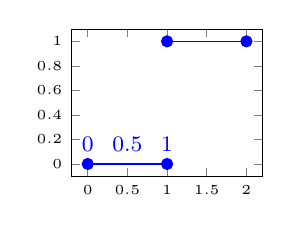
\begin{tikzpicture}
\begin{axis}[tiny]
\addplot coordinates {
	(0,0) (1,0) 

	(1,1) (2,1)}
	[pos segment=0,yshift=7pt,font=\footnotesize]
	node[pos=0] {0} 
	node[pos=0.5] {0.5} 
	node[pos=1] {1};
\end{axis}
\end{tikzpicture}
\end{codeexample}
	Here, the plot has two segments. However, all three annotation nodes are placed with |pos segment=0|.

\pgfplotsexpensiveexample
\begin{codeexample}[]
\begin{tikzpicture}
\begin{axis}
\addplot3[contour gnuplot,domain=0:1] {x*y}
	[sloped,
	 allow upside down,
	 pos segment=2,
	 every node/.style={yshift=7pt}]
	node[pos=0] {0} 
	node[pos=0.5] {0.5} 
	node[pos=1] {1}
	;

\end{axis}
\end{tikzpicture}
\end{codeexample}
	This plot has four segments (which are generated automatically by the plot handler). The annotation nodes are placed
	on the third segment, where |sloped| causes them to be rotated, |allow upside down| improves the rendering of the `$0$', and |every node/.style| install a shift in direction of the normal vector (see the documentation of |sloped| for details).
\end{key}

Occasionally, one wants to place a node using |pos| \emph{and} one wants to typeset the coordinates of that point inside of the node. This can be accomplished using |\pgfplotspointplotattime|:
\begin{commandlist}{\pgfplotspointplotattime,\pgfplotspointplotattime\marg{fraction}}
	This command is part of the |pos=|\marg{fraction} implementation: it defines the current point of \pgfname\ to \meta{fraction} of the current plot. Without an argument in curly braces, |\pgfplotspointplotattime| will take the current argument of the |pos| key.

	Thus, the command computes the basic \pgfname\ coordinates -- but it also returns the \emph{logical} coordinates of the resulting point into the following keys:
\begin{pgfplotsxykeylist}{/data point/\x}
	After |\pgfplotspointplotattime| returns, these macros contain the $x$, $y$, and $z$ coordinates of the resulting point. They can be used by means of |\pgfkeysvalueof{/data point/x}|, for example.
\begin{codeexample}[]
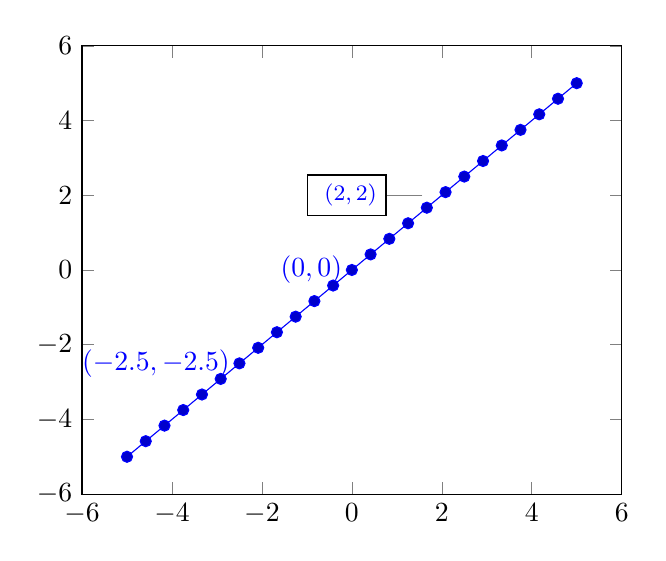
\begin{tikzpicture}
	\begin{axis}
\addplot {x} 
	[left,/pgf/number format/relative=0]
node[pos=0.5] {%
  \pgfplotspointplotattime
  $(\pgfmathprintnumber
  		{\pgfkeysvalueof{/data point/x}},
    \pgfmathprintnumber
		{\pgfkeysvalueof{/data point/y}})$
}
node[pos=0.25] {%
  \pgfplotspointplotattime
  $(\pgfmathprintnumber
  		{\pgfkeysvalueof{/data point/x}},
    \pgfmathprintnumber
		{\pgfkeysvalueof{/data point/y}})$
}
node[pos=0.7,pin=180:{%
  \pgfplotspointplotattime{0.7}
  $(\pgfmathprintnumber
  		{\pgfkeysvalueof{/data point/x}},
    \pgfmathprintnumber
		{\pgfkeysvalueof{/data point/y}})$
}] {}
	;
	\end{axis}
\end{tikzpicture}
\end{codeexample}

	In the example above, three nodes have been placed using different |pos=| arguments. Invoking |\pgfplotspointplotattime| inside of the associated node's body checks if |pos| already has a value and uses that value. The third node displays the coordinates inside of a |pin|. Due to internals of \tikzname, the |pin| knows nothing about the |pos=0.7| argument of its enclosing |node|, so we need to replicate the `|0.7|' argument for |\pgfplotspointplotattime{0.7}|. The |/pgf/number format/relative=0| style causes the number printer to round relative to $10^0$ (compare against the same example without this style).

	In case you have |symbolic x coords| (or any other |x coord inv tafo| which produces non-numeric results), the output stored in |/data point/x| will be the symbolic expression:
\begin{codeexample}[]
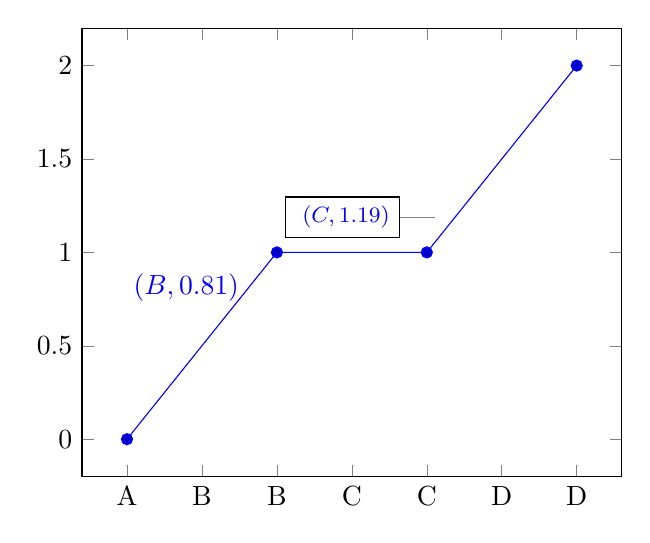
\begin{tikzpicture}
	\begin{axis}[symbolic x coords={A,B,C,D}]
\addplot coordinates {(A,0) (B,1) (C,1) (D,2)} 
	[left]
node[pos=0.3] {%
  \pgfplotspointplotattime
  $(\pgfkeysvalueof{/data point/x},
    \pgfmathprintnumber
		{\pgfkeysvalueof{/data point/y}})$
}
node[pos=0.7,pin=180:{%
  \pgfplotspointplotattime{0.7}
  $(\pgfkeysvalueof{/data point/x},
    \pgfmathprintnumber
		{\pgfkeysvalueof{/data point/y}})$
}] {}
	;
	\end{axis}
\end{tikzpicture}
\end{codeexample}
	\noindent In that specific case, you have to avoid |\pgfmathprintnumber| since the argument is \emph{no} number. Note that |symbolic x coords| cannot return fractions between, say, $A$ and $B$ as you would expect. However, the point will still be placed at the fractional position (unless you have a |scatter| or |bar| plot).

	 The computation of coordinates for the |pos| feature is computationally expensive for plots with many points. To reduce time, \PGFPlots\ will cache computed values: invoking the command |\pgfplotspointplotattime| multiple times with the same argument will reuse the computed value.
\end{pgfplotsxykeylist}


\end{commandlist}

}


\subsubsection{Placing Decorations on Top of a Plot}
{
\tikzset{external/figure name/.add={}{decorations_}}%

\tikzname\ comes with the powerful \declareandlabel{decorations} library (or better: set of libraries). Decorations allow to replace or extend an existing path by means of fancy additional graphics. An introduction into the decorations functionality of \tikzname\ is beyond the scope of this manual and the interested reader should read the associated section in~\cite{tikz}.

This section shows how to use decorations to enhance plots in \PGFPlots.
Suppose you have some graphics for which you would like to add ``direction pointers'':
\begin{codeexample}[]
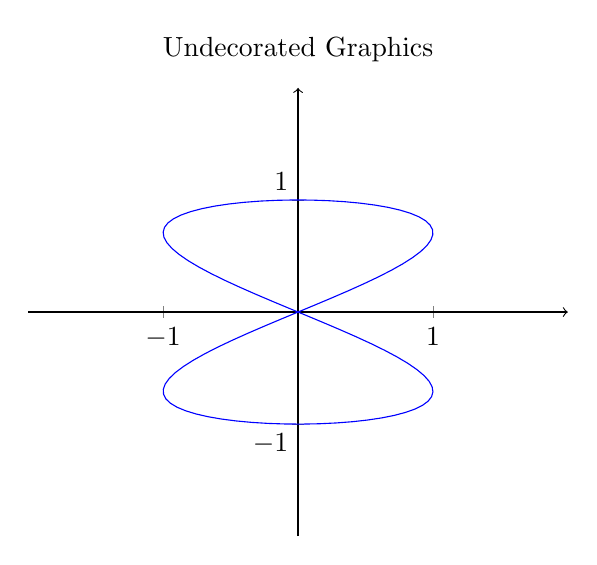
\begin{tikzpicture}[]
% An undecorated graphics with a lot of 
% pretty-printing styles:
\begin{axis}[
	axis lines=middle,
	title=Undecorated Graphics,
	xmin=-2, xmax=2, ymin=-2, ymax=2,
	xtick={-1,1}, ytick={-1,1},
	% this disables the standard 
	% tick label *text* (but not the line)
	yticklabel=\ ,
	extra description/.code={
		% this generates custom y labels to implement 
		% individual styles for every tick:
		\node[below left] at (axis cs:0,-1) {$-1$};
		\node[above left] at (axis cs:0,1) {$1$};
	},
	axis line style={->},
  ]
  \addplot[blue,samples=100,domain=0:2*pi]
	({sin(deg(2*x))}, {sin(deg(x))});
\end{axis}
\end{tikzpicture} 
\end{codeexample}
\noindent Our aim is to add short pointers indicating the direction of the parameterization. 

The solution is to use |\usetikzlibrary{decorations.markings}| and a decoration inside of |\addplot|:
% \usetikzlibrary{decorations.markings}
\begin{codeexample}[]
% requires \usetikzlibrary{decorations.markings}
\begin{tikzpicture}[]
% Same as in previous example, but with decorations:
\begin{axis}[axis lines=middle,
	title=Decorated Graphics,
	xmin=-2, xmax=2, ymin=-2, ymax=2,
	xtick={-1,1}, ytick={-1,1},
	% this disables the standard 
	% tick label *text* (but not the line)
	yticklabel=\ ,
	extra description/.code={
		% this generates custom y labels to implement 
		% individual styles for every tick:
		\node[below left] at (axis cs:0,-1) {$-1$};
		\node[above left] at (axis cs:0,1) {$1$};
	},
	axis line style={->},
  ]
  \addplot[blue,samples=100,domain=0:2*pi,
	postaction={decorate},% ------
	decoration={markings, % ------
		 mark=at position 0.25 with {\arrow{stealth}},
		 mark=at position 0.5  with {\arrow{stealth}},
		 mark=at position 0.75 with {\arrow{stealth}}}
	]
	({sin(deg(2*x))}, {sin(deg(x))});
\end{axis}
\end{tikzpicture} 
\end{codeexample}
	\noindent The only changes are in the option list for |\addplot|: it contains a \declareandlabel{postaction}|={|\declareandlabel{decorate}|}| which activates the decoration (without replacing the original path) and some specification \declareandlabel{decoration} containing details about how to decorate the path.

	A discussion of details of the |decorations| libraries is beyond the scope of this manual (see~\cite{tikz} for details), but the main point is to add the required decorations to |\addplot| and its option list.
	
}

